\documentclass{paper}
\usepackage{float}
\usepackage{wrapfig}
\usepackage{hyperref}
\usepackage{amsmath,amsfonts,graphicx}
\usepackage{subcaption}
\usepackage{tikz}
\usepackage{multirow}
\usetikzlibrary {shapes.geometric}
\usetikzlibrary {positioning}

\begin{document}

\section{David Tolpin, BGU: Deep Bayesian models of multivariate time series for anomaly detection}

\subsection{Innovation}

Evolving state of OT environments  is monitored through collection and
streaming of multivariate time series. Advances in time series forecasting due
to adoption of multilayer recurrent neural network architectures make it
possible to forecast in high-dimensional time series, and identify and
classify novelties (anomalies) early, based on subtle changes in the trends.
However, mainstream approaches to multi-variate time series predictions do not
handle well cases when the ongoing forecast must include uncertainty and shape
(possibly multimodal) of future distributions of observations. Stochastic
latent variable variants of high-dimensional time series models where
proposed, but so far have had to rely on sampling to account for uncertainty,
limiting the performance of data handling. In addition, main-stream methods of
multivariate time series forecasting are not well-suited for handling missing
data, while transient unavailability of some of the data sources (e.g. when a
sensor stops working, or a transport channel malfunctions) is  a common case
with monitoring of complex systems.  Combining state-of-the-art methods of
forecasting in high-dimensional time series (based on neural-network
architectures) with full Bayesian handling of uncertainty (e.g. with help of
deep probabilistic programming systems such as Pyro, Tensorflow Probability,
and others) will allow to achieve robust forecasting (a precondition for
anomaly detection) in high-dimensional time series with missing data.
Representing future states as inferred posterior probability distributions
will allow to identify and classify anomalies (e.g. hardware failures,
software errors, communication, malicious activity, cyberattacks, e.t.c.) on a
higher level of model abstraction — the latent variables of the model, and
achieve finer and more robust anomaly detection and characterization.

\subsection{Concept}

\begin{figure}
\begin{subfigure}{.64\textwidth}
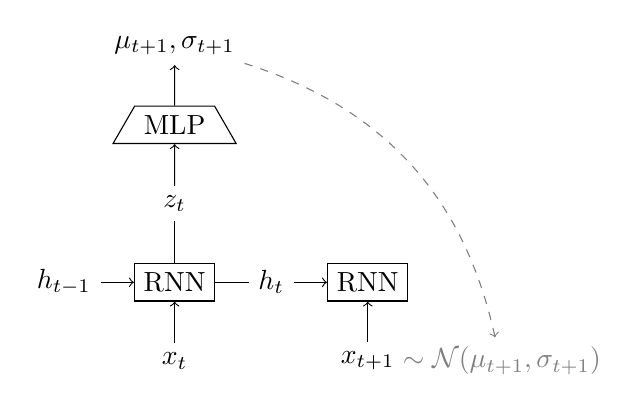
\begin{tikzpicture}
\node [rectangle, draw] (rnn) {RNN};

\node (z_t) [above of=rnn] {$z_t$};
\node [trapezium, draw] (mlp) [above of=z_t] {MLP};
\draw [-] (rnn) to (z_t);
\draw [->] (z_t) to (mlp);

%output
\node (musigma) [above of=mlp] {$\mu_{t+1}, \sigma_{t+1}$};
\draw [->] (mlp) to (musigma);

%input
\node (x_t) [below of=rnn] {$x_t$};
\draw [->] (x_t) to (rnn);

\node (h_tm1) [left=12pt of rnn] {$h_{t-1}$};
\draw [->] (h_tm1) to (rnn);

\node (h_t) [right=12pt of rnn] {$h_{t}$};
\draw [-] (rnn) to (h_t);

\node (rnnnext) [rectangle, draw, right=12pt of h_t] {RNN};
\draw [->] (h_t) to (rnnnext);

\node (xnext) [below of=rnnnext] {$x_{t+1}$};
\draw [->] (xnext) to (rnnnext);

%sampling
\node (N) [gray,right=-4pt of xnext] {$\sim \mathcal{N}(\mu_{t+1}, \sigma_{t+1})$};
\draw [->, dashed,gray] (musigma) to [bend left] (N);

\end{tikzpicture}
\caption{Conventional model}
\label{fig:dt-conventional-model}
\end{subfigure}%
\begin{subfigure}{.36\textwidth}
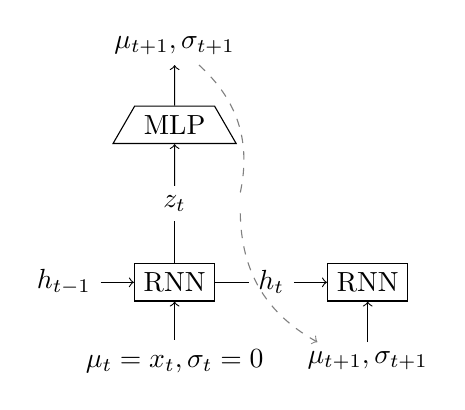
\begin{tikzpicture}
\node [rectangle, draw] (rnn) {RNN};

\node (z_t) [above of=rnn] {$z_t$};
\node [trapezium, draw] (mlp) [above of=z_t] {MLP};
\draw [-] (rnn) to (z_t);
\draw [->] (z_t) to (mlp);

%output
\node (musigma) [above of=mlp] {$\mu_{t+1}, \sigma_{t+1}$};
\draw [->] (mlp) to (musigma);

%input
\node (x_t) [below of=rnn] {$\mu_t=x_t,\sigma_t=0$};
\draw [->] (x_t) to (rnn);

\node (h_tm1) [left=12pt of rnn] {$h_{t-1}$};
\draw [->] (h_tm1) to (rnn);

\node (h_t) [right=12pt of rnn] {$h_{t}$};
\draw [-] (rnn) to (h_t);

\node (rnnnext) [rectangle, draw, right=12pt of h_t] {RNN};
\draw [->] (h_t) to (rnnnext);

\node (xnext) [below of=rnnnext] {$\mu_{t+1}, \sigma_{t+1}$};
\draw [->] (xnext) to (rnnnext);

\node (F) [right=12pt of z_t] {};
\draw [-,dashed,gray] (musigma) to [bend left] (F);
\draw [->,dashed,gray] (F) to [bend right] (xnext);

\end{tikzpicture}
\caption{Model with uncertainty propagation}
\label{fig:dt-uncertainty-propagation}
\end{subfigure}
\caption{Time series models}
\label{fig:dt-time-series-models}
\end{figure}

There is a range of neural recurrent models of varying complexity to
deal with time series prediction. Most models include a
recurrent unit which threads the state through the time steps,
accepts data as inputs and produces next step predictions as
outputs. The simplest model is an RNN with a fully-connected
readout layer to produce predictions (Figure~\ref{fig:dt-conventional-model}).
RNN can be based on GRU, LSTM, or another variant, and is often
multi-layer. Architectures  may also include intermediate modules and sampling-based variational layers.

Variants are stochastic RNNs, variational RNNs, etc. The
overall architecture stays almost the same, with more
connections, intermediate modules and sampling-based variational
layers.

\paragraph{Input and Output} This architecture normally accepts data vectors and outputs vectors of predictions of means and standard deviations (the output is twice as wide as the input). Then, to generate a forecast, one samples from $$\mathcal{N}(\mu, \sigma)$$ for each component, and feeds the sample as the input to the next time step.

\paragraph{Training} The model is trained to maximize probability of prediction. In the most basic case, a single step is predicted for each time step in the series. If a series has 10 steps, then steps 1 .. 9 are input, and the steps 2 .. 10 are truth. The network is trained to
minimize negative log probability of true observations given
predictions under variational approximation of product of
Gaussians. 

\paragraph{Novelty detection} After training, the model is used to produce predictions of future observations. There are two related but different phenomena indication a novelty (anomaly) in time series behavior: \begin{enumerate}
    \item Predicted volatility of the time series is high, that is, future observations can only be forecast uncertainly (with high variance). 
    \item Probability of actual observations, when observed, given a prediction from a past state, is low.
\end{enumerate}

Either phenomenon, or both of them, can be used to alert about novelties in the time series. In recurrent neural network architectures, the hidden state ($h_t$ in Figure~\ref{fig:dt-time-series-models}) can be used to identify and classify anomalies.

However, the basic scheme outlined above poses difficulty in applications with high-dimensional time series and partially missing observations. Sampling based uncertainty assertion impacts performance, and missing observations are often imputed in \textit{ad hoc} manner. An architecture which
incorporates confidence about data and in which observed and
predicted data are interchangable is  highly, desirable. For example,k if out of 5 components 3 were
measured and 2 predicted from an earlier step we want to input
them both into the next time step for further forecasting. In
addition, the model architecture should be capable of robust uncertainty prediction and benefit from training with multiple steps of out-of-sample data. To achieve these objectives, we propose the following changes (Figure~\ref{fig:dt-uncertainty-propagation}):

\begin{enumerate}
\item The input, as well as the output, is a vector of means followed
by standard deviations. If the data has 5 components, the input
will be 10-dimensional. For observed data --- measurements
present at the current time step --- the standard deviation is
zero. For missing data the input is mean and standard deviation
as predicted from the previous time step.

\item Since we introduce confidence into the input, we cannot train
the network myopically, on a single step prediction --- or the
standard deviations in the input data will always be zero, and
the network will never learn how to use them. To overcome this,
we train on multiple predicted steps. We feed each prediction,
without sampling, as input to the next step and compute the loss
as negative log probability of this number of future points versus our prediction.
\end{enumerate}

To illustrate, given the data set of 5 dimensions, the input has 10
dimensions. If we train with 3 time steps lookahead, the ground
truth will be a matrix of size 3x5. The prediction against
which the likelihood of this ground truth is computed will be
a matrix of size 3x10. Intuitively, we would expect the
predicted standard deviation to increase along the time axis
for each component.

The ability of Bayesian forecasting with uncertainty, in the form of a multivariate Gaussian distributions, far into the future, opens opportunity for application for more robust novelty detection
approaches. Instead of detecting novelty based on log probability of observations given predictions from the past, which is prone to false positives due to observation noise, novelties can be detected and analysed by comparing predictions of the same time point from different points in the past. In this case, KL-divergence between predictions provide a theoretically sound and robust mechanism for detection of anomalies~\cite{10.1145/3297280.3297414}, and is in particular relevant for monitoring of large OT environments with high dimensionality of time series and occasional missing values and heteroskedastic noise.

\subsection{Proposed R\&D Program}

Monitoring of complex systems based on multivariate time series meets challenges in adapting a general algorithm to  domain-specific properties of the particular system~\cite{DBLP:conf/iccst/DymshitsMT17}. As the \textbf{first step}, the structure and scale of time series emerging in monitoring of power plants, and relevance of various components of the time series for novelty detection, in particular related to cybersecurity, has to be analyzed. As compelling as it may sound, feeding all of the available observations in their raw form to a general model will unlikely to result in robust novelty detection. Hence, we propose to start with empirical evaluation of smoothing and forecasting capabilities of existing multi-variate time series model on different representations of the time series. Conventional neural multivariate time series models, while having drawbacks, will aid in selecting the right representation of the data, which can be assessed by the quality of forecasting, which should be consistently high in normal operation and decrease in presence of otherwise observed disturbances (hardware and operational failures, cybersecurity attacks, etc.). Using established modelling approaches as a test bench, we will be able to come with an appropriate representation of the time series emerging in power infrastructure monitoring.

\textbf{Following this}, we propose implementing and evaluating the deep Bayesian model, as outlined above, in its basic form, implemented as an extension of an established time series prediction architecture. By doing so, we will be able to use the earlier architecture as a comparison baseline, and assess improvements due to Bayesian handling of uncertainty by comparing performance of detection and identification of novelties. Both recorded real and simulated novelties can be used for this stage.

Provided that the previous step succeeds, research on classification and characterization of novelties can be commenced, which is, in a sense, orthogonal to time series forecasting, and is based on extending the base model with modules using the internal state of the recurrent network to learn to recognize or characterize types and features of novelties. This layered plan of the research allows to go back to earlier steps (data representation, extension of time series models with Bayesian handling of uncertainty, advanced techniques for novelty identification and characterization) in case results of a later step uncover obstacles introduced earlier and require changes in theory or implementation. 

\end{document}
